\section{\bt{System Overview}{系统概览}}
\label{sec:overview}
\bi{\system\ sits between agents and a SQL database, PostgreSQL in our prototype (Figure~\ref{fig:architecture}). It exposes tool-style HTTP endpoints for listing and describing tables, finding and checking join paths, looking up metric definitions (\code{find\_metric}), and running SQL (\code{run\_sql}); agents submit final answers with the query references and arithmetic that produced them, so the middleware records the provenance of every answer. An in-memory store keeps versioned definitions, join paths, grain entries, check results, and evidence. Version detection reads table fingerprints, DML statistics, and an ETL batch log; in same-snapshot mode, statement-level triggers maintain transactional table versions (Section~\ref{sec:snapshot}). The middleware is about 6,600 lines of Rust with 40 unit and integration tests.}
{\system\ 位于智能体与 SQL 数据库之间，原型使用 PostgreSQL（图~\ref{fig:architecture}）。它通过工具式 HTTP 接口提供列出和描述表、查找与检查连接路径、查找指标定义（\code{find\_metric}）以及执行 SQL（\code{run\_sql}）等功能；智能体提交最终答案时附上产生答案的查询编号和算式，因此中间件为每个答案记录溯源。内存知识库保存版本化的定义、连接路径、粒度条目、检查结果和证据。版本检测读取表指纹、DML 统计和 ETL 批次日志；在同快照模式下，语句级触发器维护事务性表版本（第~\ref{sec:snapshot} 节）。中间件约 6,600 行 Rust 代码，含 40 个单元与集成测试。}

\begin{figure*}[t]
\centering
% Vector drawing generated by tools/figures/architecture.py; rerun it after changing the figure.
\ifbilingual
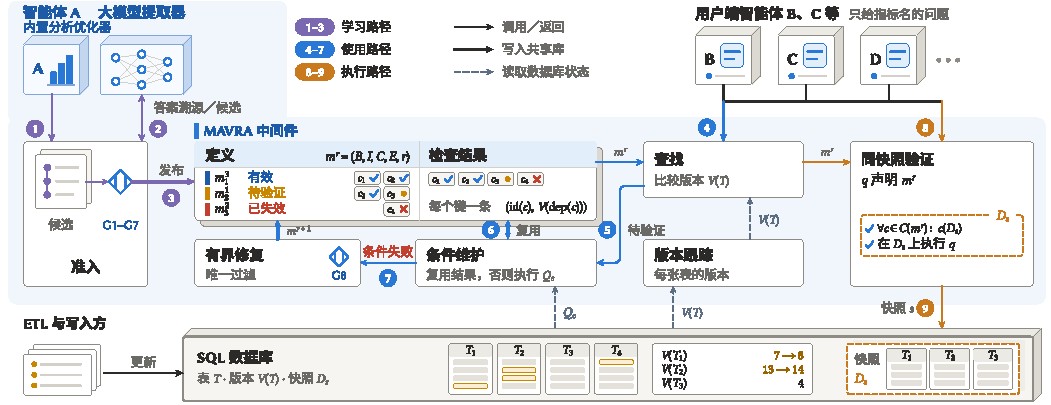
\includegraphics[width=\textwidth]{figures/architecture-zh}
\else
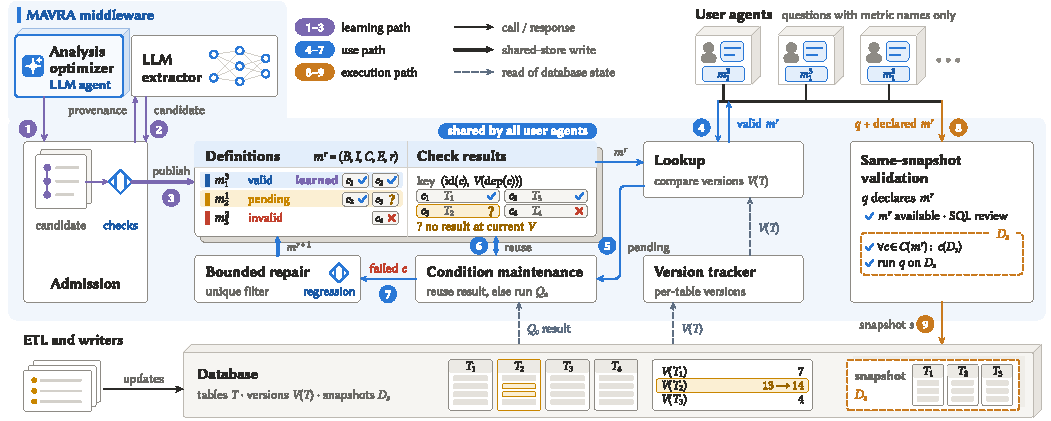
\includegraphics[width=\textwidth]{figures/architecture}
\fi
\caption{\bt{\system\ overview: a user agent's two requests across the three modules. Use path (1--5): a text request names a metric; request handling reads its definition from the shared store, maintenance first revalidates a definition whose tables changed, and only a valid revision is returned. Execution path (6--8): an SQL request declares that revision; same-snapshot validation checks its conditions on the query's snapshot and runs the query there. Learning path: the built-in analysis optimizer, an LLM agent, learns the definitions that admission publishes.}{\system\ 概览：用户端智能体的两种请求在三个模块之间的流转。使用路径（1--5）：文本请求给出指标名；请求处理从共享知识库读取定义，所读表有变化的定义先经维护重验证，只返回有效修订。执行路径（6--8）：SQL 请求声明该修订；同快照验证在查询的快照上核对其条件并在其上执行查询。学习路径：内置分析优化器（大模型智能体）学习定义，经准入后发布。}}
\label{fig:architecture}
\Description{A user agent on the left asks in text for the return amount in May and later sends SQL that declares revision 2 of that definition. Inside the MAVRA middleware sit three modules side by side: request handling with lookup and same-snapshot validation; the shared store with definitions (return amount pending, store revenue valid) and check results kept per table version; and learning and maintenance with the built-in analysis optimizer, an LLM agent, and maintenance, which rechecks, repairs, or invalidates. Blue steps 1 to 5 run from the agent to lookup, from the store to lookup, from the pending definition to maintenance, from maintenance back into the store, and from lookup back to the agent with a valid definition. Orange steps 6 to 8 run from the agent's SQL query to same-snapshot validation, between validation and the check results, and back to the agent with the query result. A thick violet arrow publishes learned definitions into the store. Below, a SQL database holds the query's snapshot, the table versions, in which store\_returns moved from 14 to 15, and the tables; ETL writers update it, validation runs the query on the snapshot, maintenance runs check queries, and the store reads table versions.}
\end{figure*}


\bi{A definition moves through three paths. On the \emph{learning path}, \system's built-in analysis optimizer, an LLM agent, answers a question whose business meaning is stated explicitly; if an independent judge accepts the answer, an offline extractor turns the recorded answer provenance into a structured candidate, which the admission checks validate before publication. On the \emph{use path}, a user agent calls \code{find\_metric}; if any dependency version has changed, the lookup first runs condition maintenance and then returns the current valid revision with its fields and caveats. On the \emph{execution path}, the agent's \code{run\_sql} declares the metric keys and revisions it uses; the middleware rejects absent, invalidated, or superseded revisions, reviews the SQL against recorded grain and join requirements, and, in same-snapshot mode, checks the revisions' conditions and runs the query on one snapshot. Invalidations reach agents as notices on their next tool response. Figure~\ref{fig:lookup} follows both requests step by step, and Figure~\ref{fig:lifecycle} follows one definition through learning, maintenance, and repair.}
{一个定义经过三条路径。在\emph{学习路径}上，\system\ 内置的分析优化器（一个大模型智能体）回答一道显式给出业务含义的题目；若独立判题接受其答案，离线提取器把记录的答案溯源转成结构化候选，由准入检查验证后发布。在\emph{使用路径}上，用户端智能体调用 \code{find\_metric}；若有依赖版本变化，查找先执行条件维护，再返回当前有效修订及其字段和注意事项。在\emph{执行路径}上，智能体在 \code{run\_sql} 中声明所用的指标键和修订号；中间件拒绝不存在、已失效或已被替代的修订，按记录的粒度和连接要求审查 SQL，并在同快照模式下于同一快照上核对修订条件、执行查询。失效通过智能体下一次工具调用的返回中的通知传达。图~\ref{fig:lookup} 逐步展示这两种请求的处理，图~\ref{fig:lifecycle} 展示一个定义经历学习、维护与修复的全过程。}

